\newpage \mysection{Évaluation: Résultats et Performance}

\mysubsection{Surface de l’îlot}

Pour calculer la nouvelle surface occupée par l’îlot de sécurité, on a pris en compte premièrement la région démarquée par l’enceinte de sécurité, comme il est montré dans la figure \ref{fig:area_DCS}.

\begin{figure}[H]
	\begin{center}	
		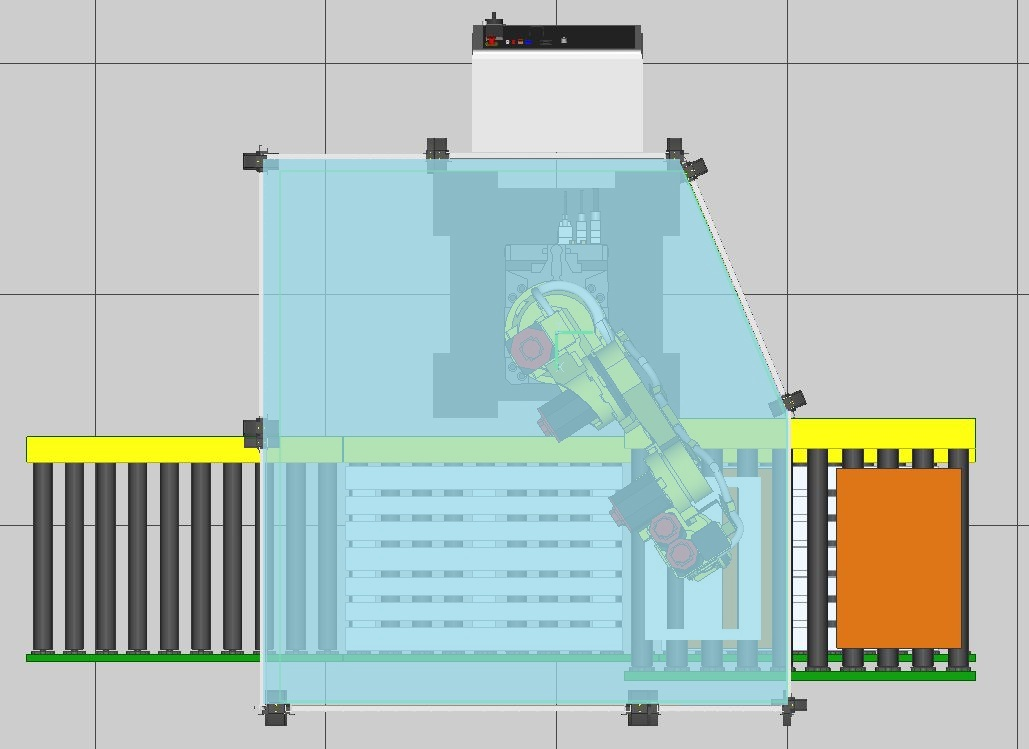
\includegraphics[width=\textwidth]{Evaluation/area_DCS.jpg}
		\caption{ Zone de travail de la cellule robotique}
		\label{fig:area_DCS}
	\end{center}
\end{figure}


De cette façon, la surface de la zone d’opération du robot qu’on a obtenu est de 5.33 $ m^2 $, ce qui correspond à une réduction 58.86\% de la surface. On peut voir qu’on a bien répondu à l’objectif principal du projet, qui était de réduire au moins par deux la surface de l’îlot. C’est donc déjà une solution fonctionnelle qui est conforme aux objectifs imposés.
De plus, même lorsque l’on prend en compte la surface occupée par tous les éléments ajoutés à la simulation, comme il est montré dans la figure \ref{fig:area_tous}, on a une valeur de 7.466 $ m^2 $ de surface. Cela montre une réduction de la surface de la cellule originale, laquelle ne prendrait en compte que la palettisation des cartons. En plus, notre solution permettra une intégration de cette cellule avec les autres opérations de l’usine, ou avec autres cellules de palettisation, si elles existent, puisque le flux de cartons est maintenant unidirectionnel.

\begin{figure}[H]
	\begin{center}	
		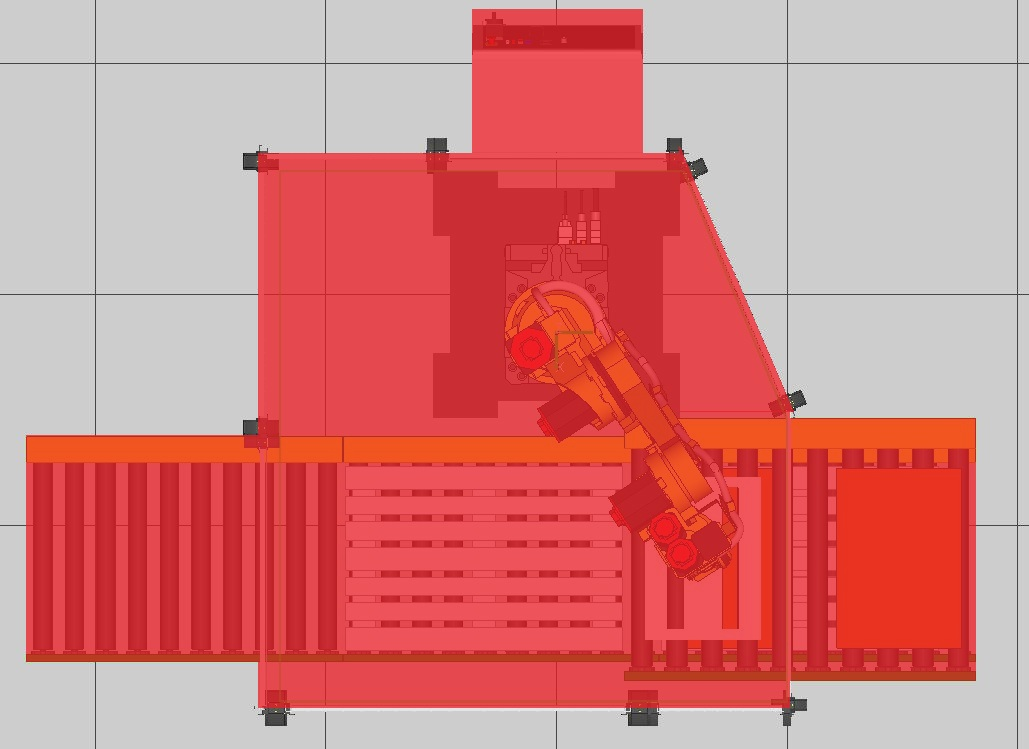
\includegraphics[width=\textwidth]{Evaluation/area_tous.jpg}
		\caption{Surface occupé par tous les éléments ajoutés dans la simulation}
		\label{fig:area_tous}
	\end{center}
\end{figure}

\mysubsection{Cadence de production}\label{cadence}

Par rapport à la cadence de production, les résultats obtenus sont très satisfaisants. Premièrement, pour avoir une évaluation plus précise de la performance, on a pris en compte la cadence qui a été fournis dans les contraintes du projet (411 cartons par heure et temps de prise/dépose des cartons par le préhenseur) et on a programmé la création des cartons pour être d’accord avec cette valeur. On a vu que, dans tous les cas, le robot attend l’arrivée d’autres cartons.
Le temps moyen d’attente par les cartons est de (4.08 $ \pm $ 0.14) s  (temps moyen en variations constatées ). Le temps d’exécution de la tâche a été évalué avec l’outil Profiler de Roboguide, trois fois pour chaque carton, en prenant soin d’éliminer les temps de déblocage des freins. Alors, le robot n’est pas seulement capable de maintenir la cadence de production, mais il permet aussi de l’augmenter. On peut augmenter la vitesse de production à 411 cartons tous les (32 $ \pm $ 1)  minutes, ce qui correspond à environ (770 $ \pm $ 24) cartons par heure. On peut augmenter de (87.3 $ \pm $ 5.8) \% la vitesse de production.
Si on considère le pire cas, quand le robot prend plus de temps pour réaliser son mouvement, il reste en attente pour le prochain carton pendant 3.76 s. Cela permet encore d’augmenter la cadence de production en 75\% (720 cartons par heure). 



\newpage
\mysubsection{Sécurité}
Dans la discussion autour de la sécurité on a proposé trois mesures pour faire face aux risques associés à l'opération de la cellule, et l’accent a été mis sur la conformité avec la norme internationale ISO 13849-1, donc il faut valider la cellule avec cette norme.
Le processus de validation de la norme, comme décrit dans la mise à jour de 2006, est basée sur le principe que le PL obtenu par une SRP/CS doit être plus grand ou égal au PL requis par la source de risque en question. Les \textit{Performance Levels} de chaque fonction, selon FANUC, sont décrits ci-dessous. 

\begin{table}[H]
	\caption{Performance Level des fonctions de sécurité vs PL requis}
	\label{tab:Performance_Level}
	\begin{tabularx}{\textwidth}{>{\centering\arraybackslash}X|>{\centering\arraybackslash}X|>{\centering\arraybackslash}X|>{\centering\arraybackslash}X}
		\textbf{Source de Risque}&
		\textbf{PLr}&
		\textbf{Solution Proposée}&
		\textbf{PL}\\
		\hline		
		Accès des palettes&
		PLd&
		Cartesian Position Check&
		PLd\\
		\hline		
		Maintenance&
		PLc&
		Fence input&
		PLe\\		
	\end{tabularx}
\end{table}

Ce tableau montre, donc, que du point de vue de la norme ISO 13849-1 notre cellule est validée.

\mysubsection{Prévision Budgétaire}

Pour faire la prévision budgétaire, on va analyser les principaux éléments présents dans la cellule. Au-dessous, on a un tableau avec l’estimation de prix de ces éléments:

\begin{table}[H]
	\caption{Estimation de prix}
	\label{tab:Estimation}
	\begin{tabularx}{\textwidth}{>{\centering\arraybackslash}X|>{\centering\arraybackslash}X}
		\textbf{Éléments}&
		\textbf{Prix}\\
		\hline
		Robot R-1000iA&
		45000 \euro\\
		Fonction de sécurité DCS&
		2000 \euro\\
		Préhenseur à ventouses$^\ast$  &
		700 \euro\\
		\hline
		\textbf{Total}&
		\textbf{47700 \euro}\\	
	\end{tabularx}

\end{table}
\begin{center}\footnotesize $^\ast $ - Tarif estimée à partir de l’informations sur l’internet
\end{center}  


Les tarifs du Robot (on considère que le Contrôleur R-30iB est inclus dans le prix total du robot de la gamme R-1000iB) et de la fonction de sécurité DCS ont été pris dans le catalogue de prix de la Fanuc, qui présente les tarifs non-contractuels pour ce projet. 
Le prix de l’outil utilisé dans le robot, le préhenseur à ventouse, a été estimé sur la base de prix de l’ensemble robot, machine et outil trouvés sur l’Internet. 
Les autres éléments de la cellule, comme les convoyeurs, la barrière de l'enceinte de sécurité et les coûts d’installation et d'intégration n’ont pas été considérées dans l’étude de budgétaire. On ne peut pas estimer avec précision le prix de ces éléments parce qu’il dépende beaucoup du modèle et du fabricant de l’élément. Le modèle, par exemple, des convoyeurs, peut dépendre des autres convoyeurs de l’usine (les convoyeurs qui acheminent les cartons à la cellule, ou les convoyeurs éventuels qui apportent les palettes vides) et et d’autres contraintes d’intégration. Cependant, on sait qu’il est nécessaire d’acheter un convoyeur pour le cartons et un autre pour les palettes, qui peut être activé par zone, et aussi les capteurs pour les contrôler. Dans le cas de l’enceinte de sécurité, on a besoin d’un modèle \flqq{} fait sur mesure\frqq{}, et donc de demander un  budget directement au fabricant pour cela.














